%%%%%%%%%%%%%%%%%%%%%%%%%%%%%%%%%%%%%%%%%%%%%%%%%%%%%%%%%%%%%%%
\section{Production and Assembly}
\label{sec:fdsp-pd-prod-assy}
%\metainfo{(Length: TDR=40 pages, TP=8 pages)}

%%%%%%%%%%%%%%%%%%%%%%%%%%%%%%%%%%
\subsection{Photon Collectors Production and Assembly}
\label{sec:fdsp-pd-prod-pc}
%\metainfo{\color{blue} Content: Cavanna/Whittington/Machado}
	
\subsubsection{\color{red}\bf Dip-Coated Light Guides}
\label{ssec:fdsp-pd-pc-prod-bar1}
\metainfo{\color{red} Content needed: (2 pages) Toups}

\subsubsection{Double-Shift Light Guides}
\label{ssec:fdsp-pd-pc-prod-bar2}

The production and assembly of the double-shift light guide modules is divided 
into separate threads for the wavelength-shifting plates and the EJ-280 light guides. 
Many of the production, quality assurance, and assembly procedures developed for the
 double-shift light guide design deployed at protoDUNE-SP will remain the same for 
the DUNE single-phase far detector.

\paragraph*{Manufacture of the WLS Plates}

Spray-coating of TPB on acrylic plates (see Figure~\ref{fig:DoubleShiftLG-SprayedPlates}).

\begin{dunefigure}[TPB-coated acrylic plates after spraying at Indiana University during fabrication of parts for protoDUNE-SP.]{fig:DoubleShiftLG-SprayedPlates}
 {TPB-coated acrylic plates after spraying at Indiana University during fabrication of parts for protoDUNE-SP.}
  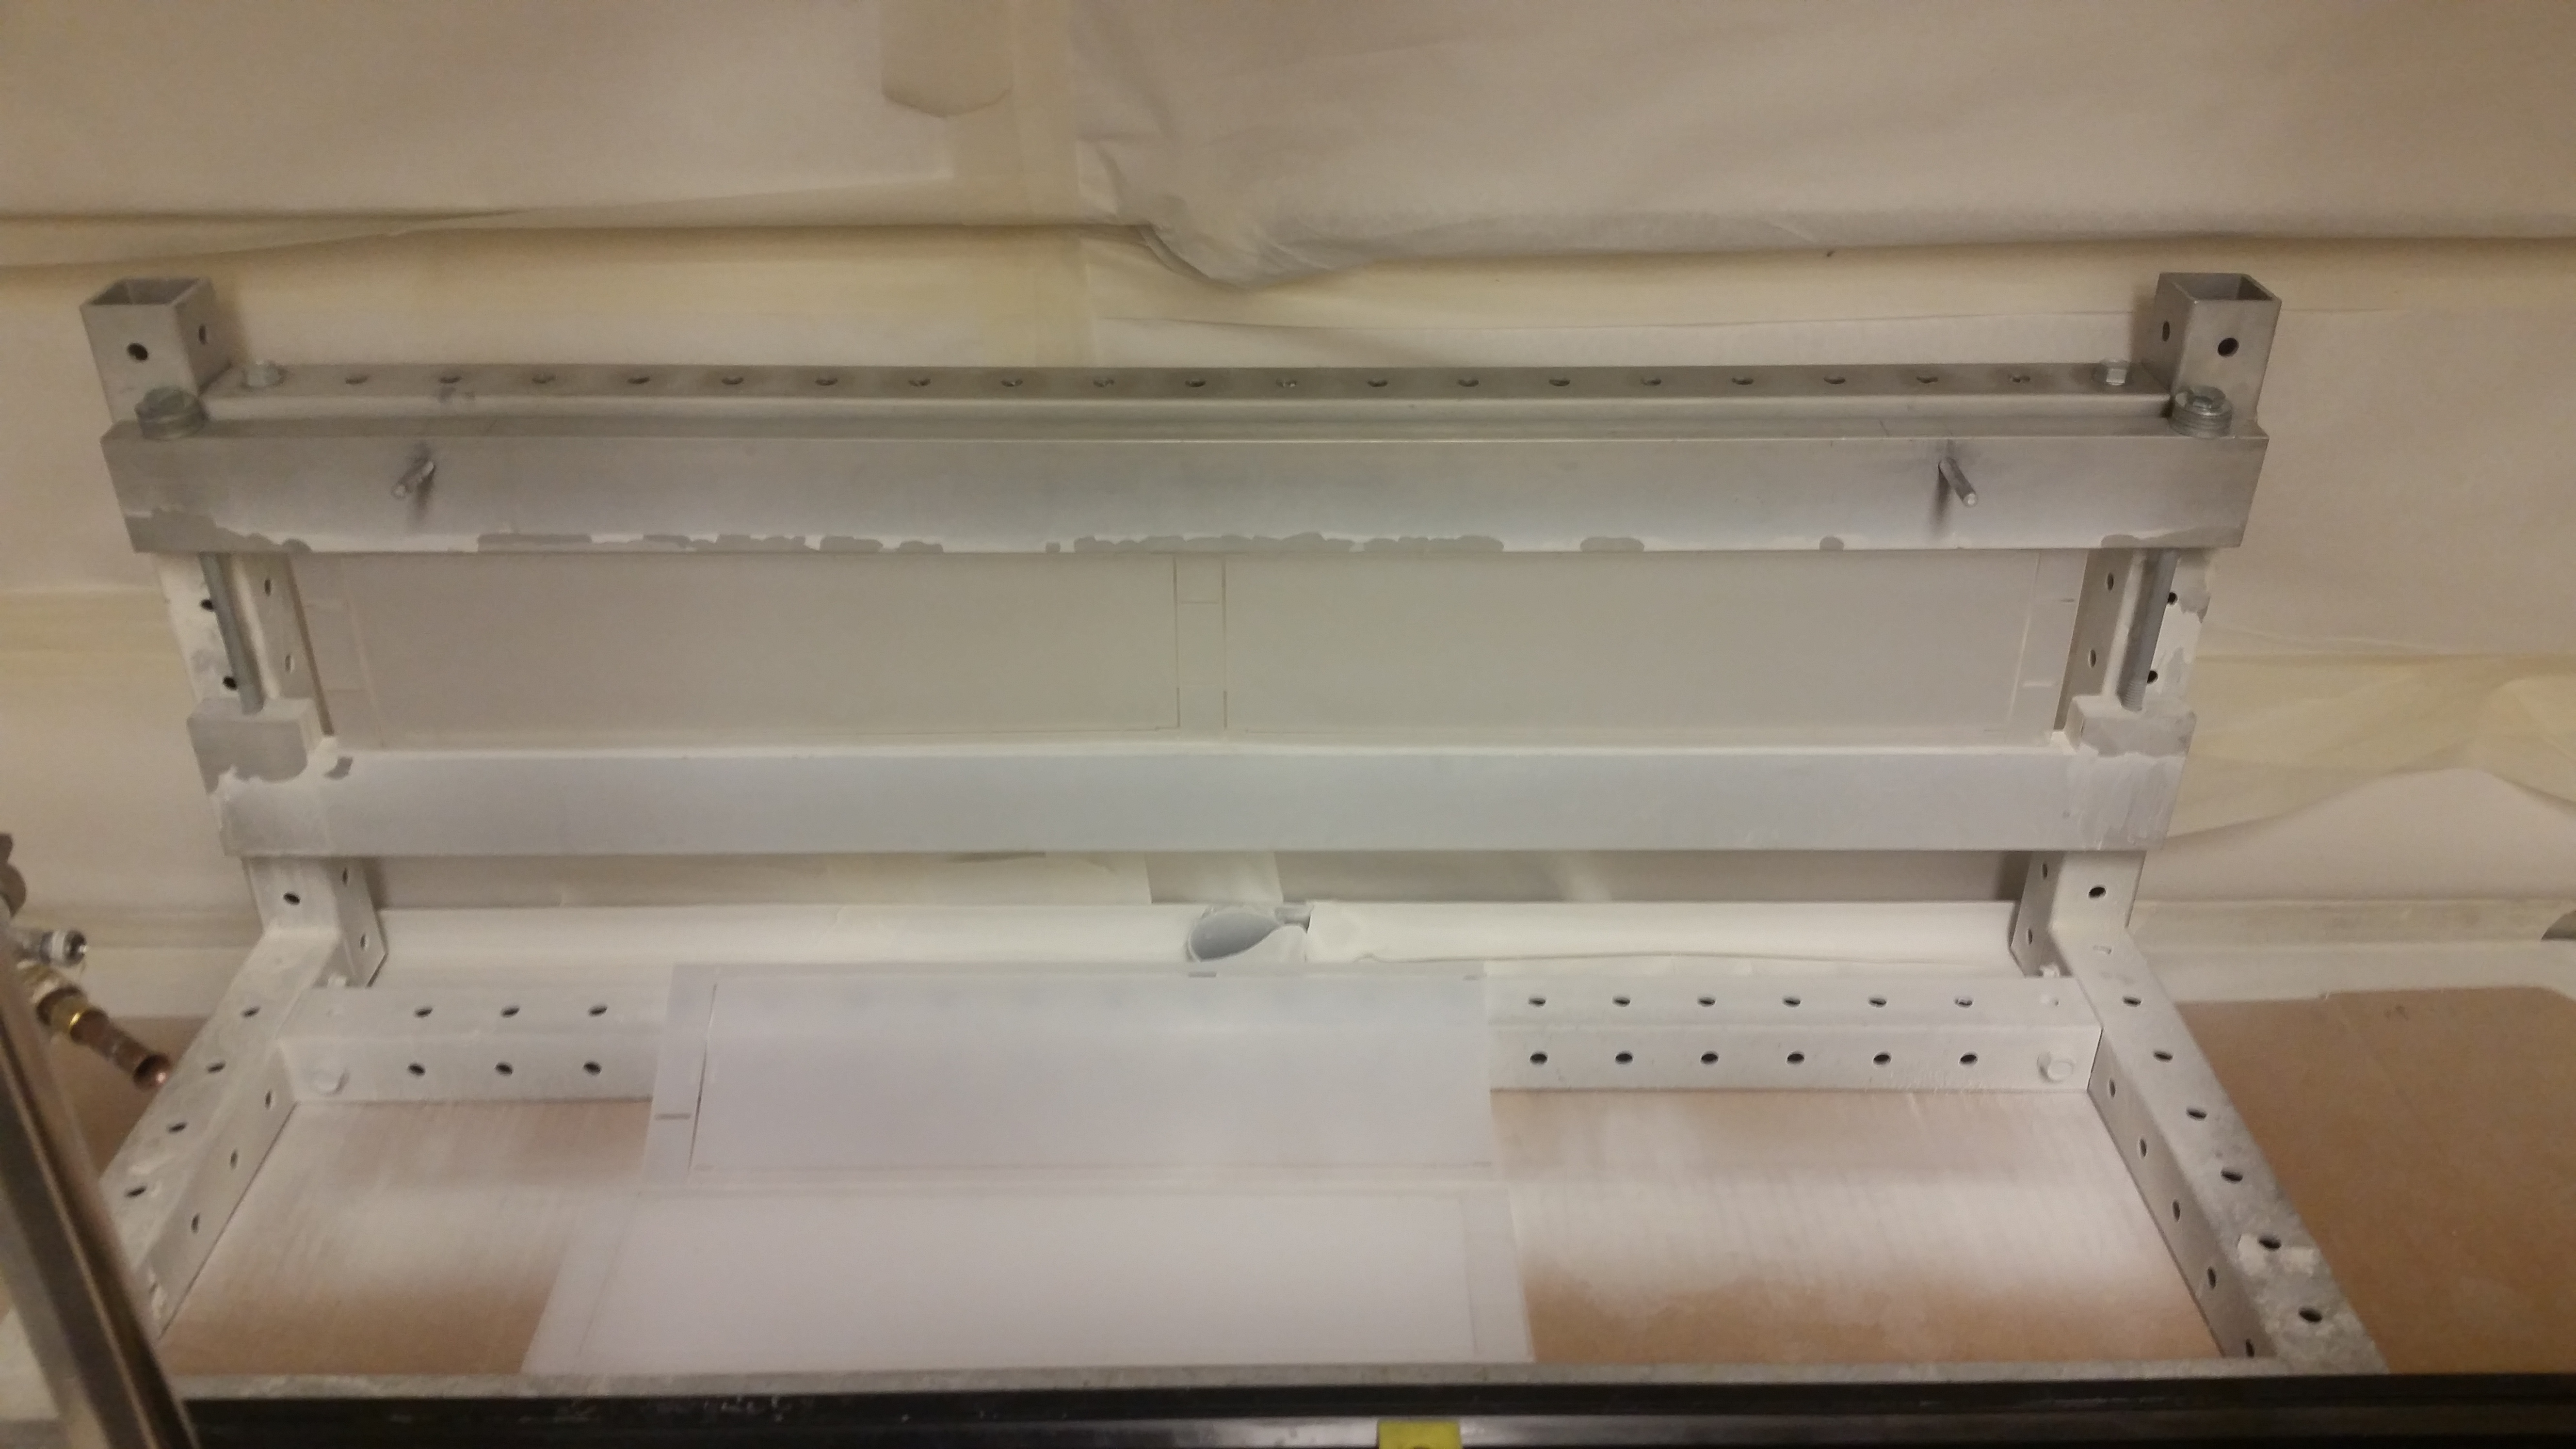
\includegraphics[width=0.7\columnwidth]{pds-DoubleShiftLG-SprayedPlates.jpg}
\end{dunefigure}

\paragraph*{QA of the WLS Plates}

VUV conversion performance measured for neighboring samples from the 
acrylic plate template using a vacuum-ultraviolet monochromator.

\paragraph*{Receipt and QA of the Light Guides}

EJ-280 light guides fabricated by Eljen Technologies. Received and scanned in a 
long dark-box using a blue LED~(Figure~\ref{fig:DoubleShiftLG-EJ280}).
 Measure conversion and transmission to the light guide ends to test attenuation. 
Direct transmission through the light guide to confirm uniformity. 
Attenuation length in liquid argon shorter than in air, but long attenuation in 
air has been shown to correspond to long attenuation in liquid argon.

\begin{dunefigure}[EJ-280 light guide within darkbox for attenuation scan QA at Indiana University (prepared for protoDUNE-SP).]{fig:DoubleShiftLG-EJ280}
{EJ-280 light guide within darkbox for attenuation scan QA at Indiana University (prepared for protoDUNE-SP).}
  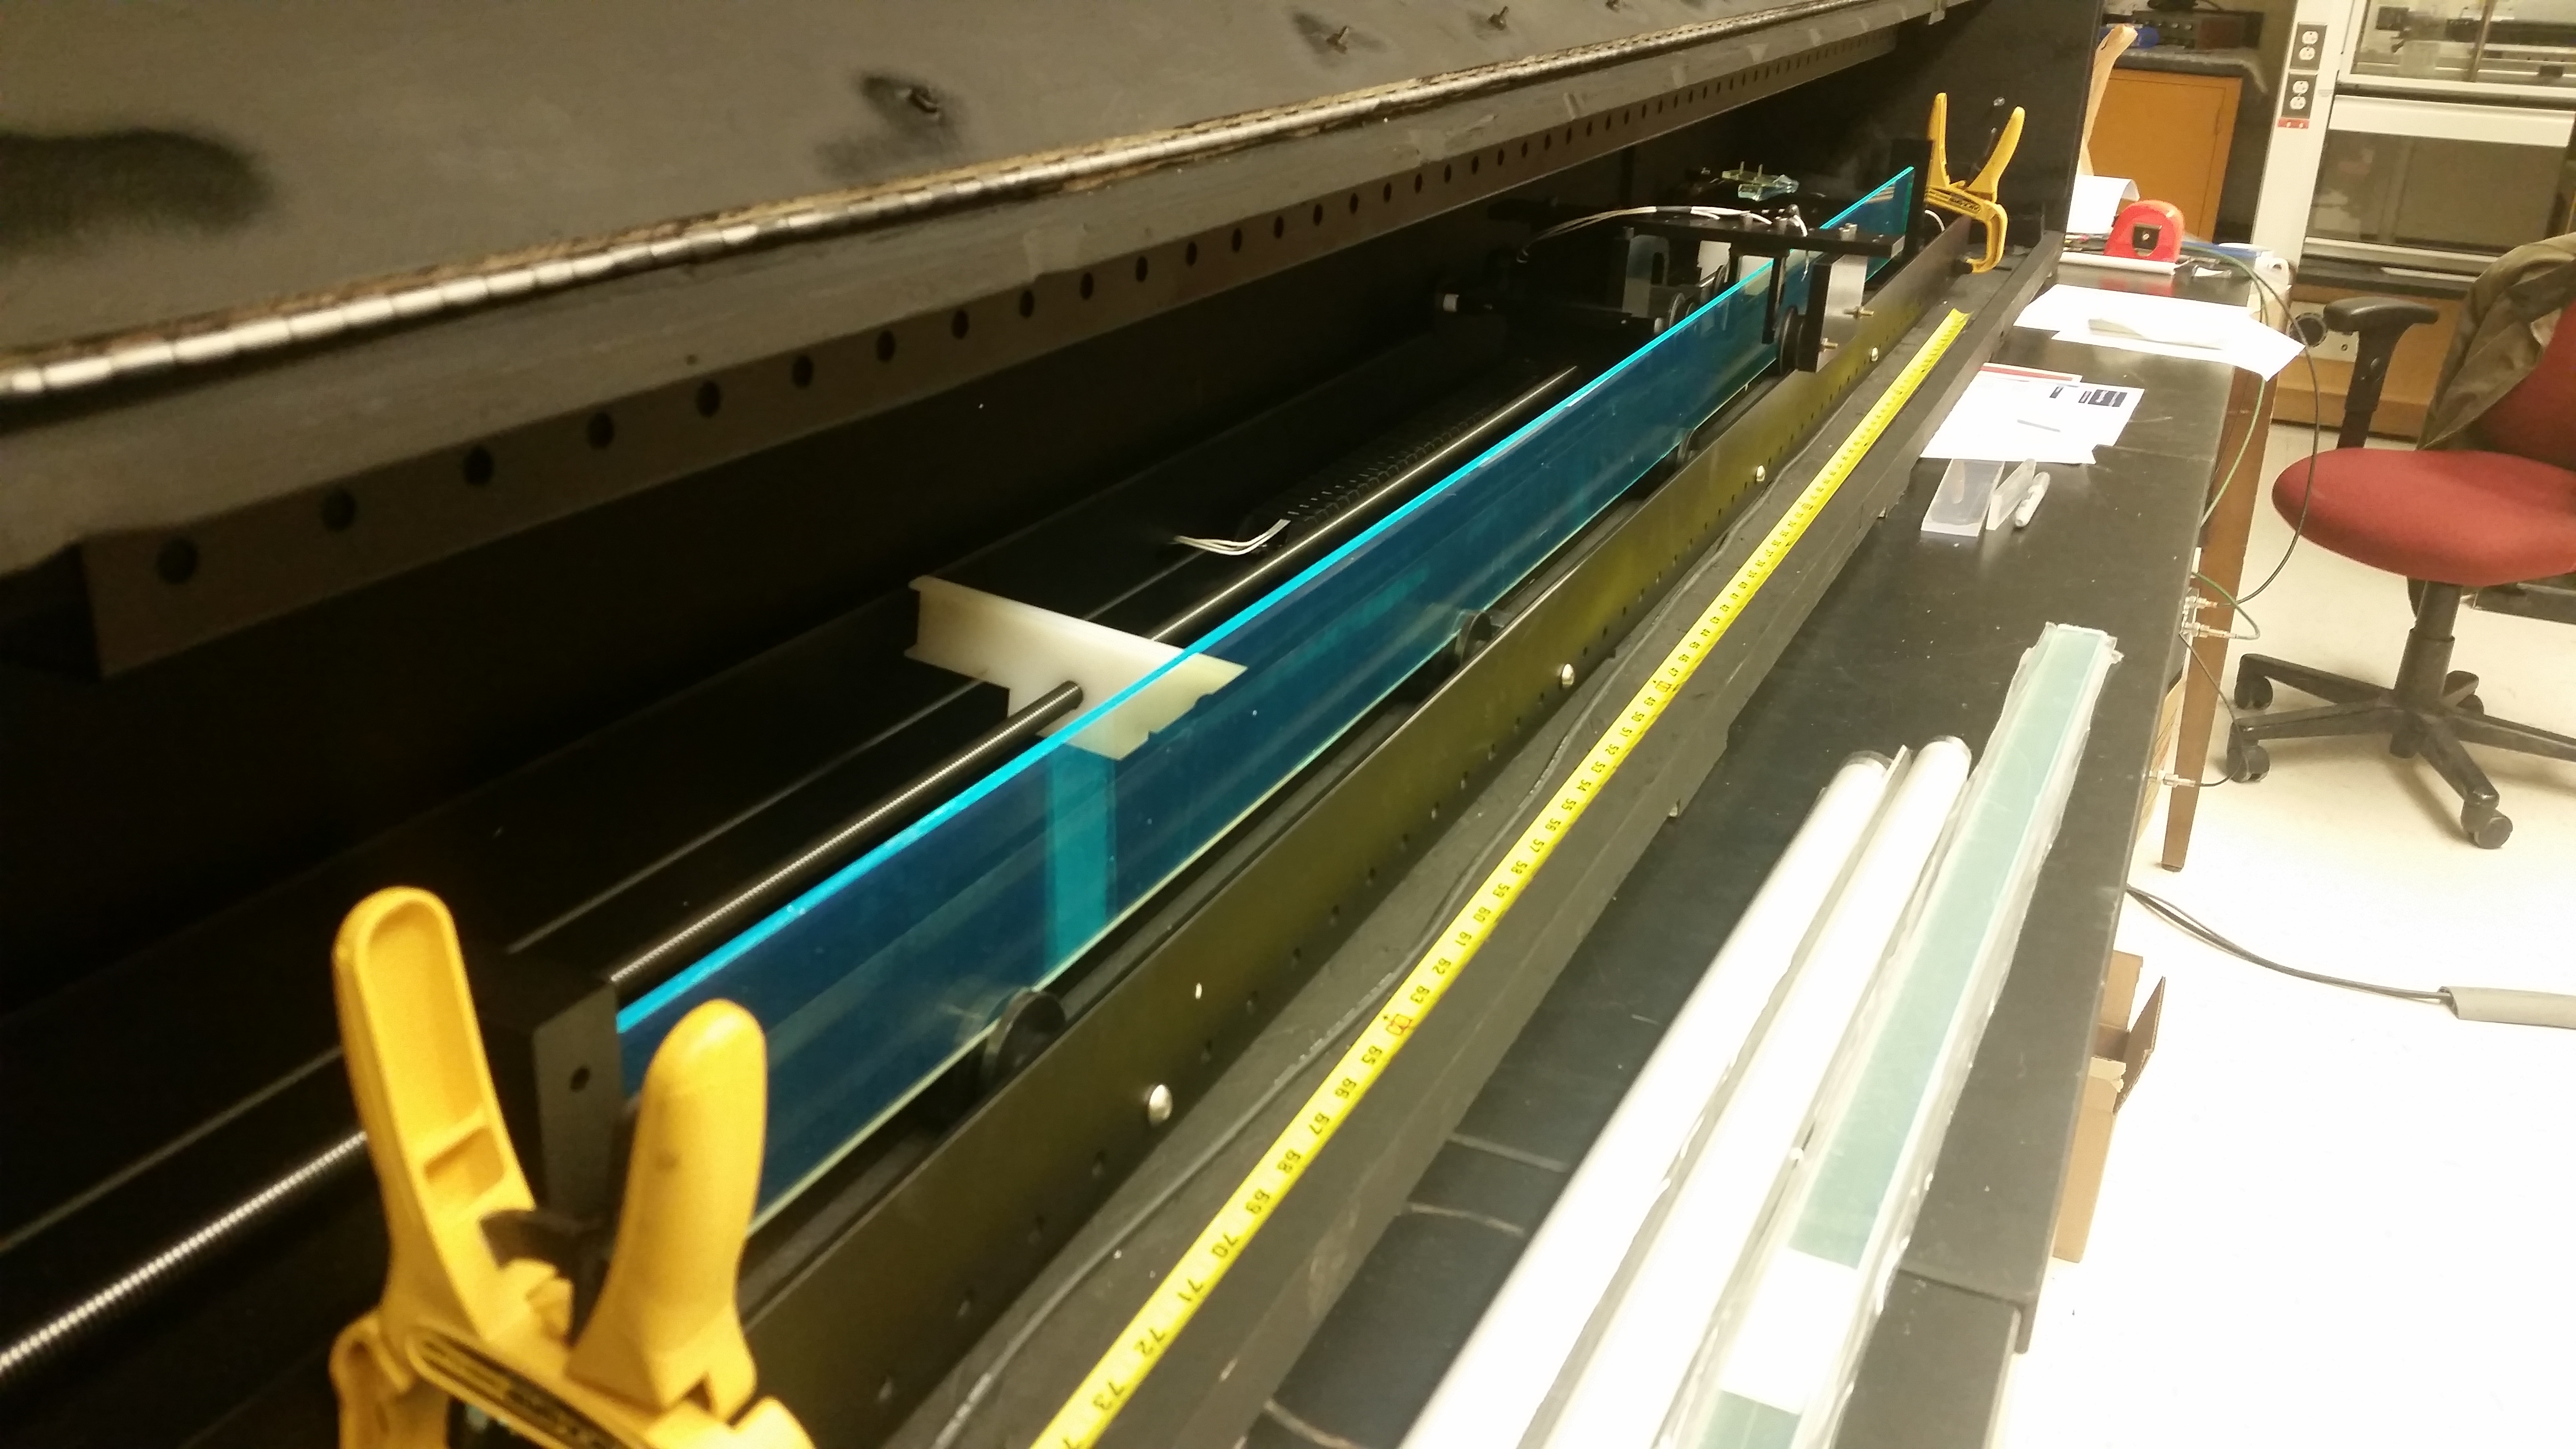
\includegraphics[width=0.6\columnwidth]{pds-DoubleShiftLG-EJ280.jpg}
\end{dunefigure}

\paragraph*{Assembly of the Double-shift Light Guide Module}

Parts are shipped to the assembly point where the EJ-280 light guide is mounted 
into the module frame and the WLS plates are attached.

\begin{dunefigure}[Mounting of the WLS plates to the EJ-280 bar.]{fig:DoubleShiftLG-PlateMounting}
{Mounting of the WLS plates to the EJ-280 bar.}
  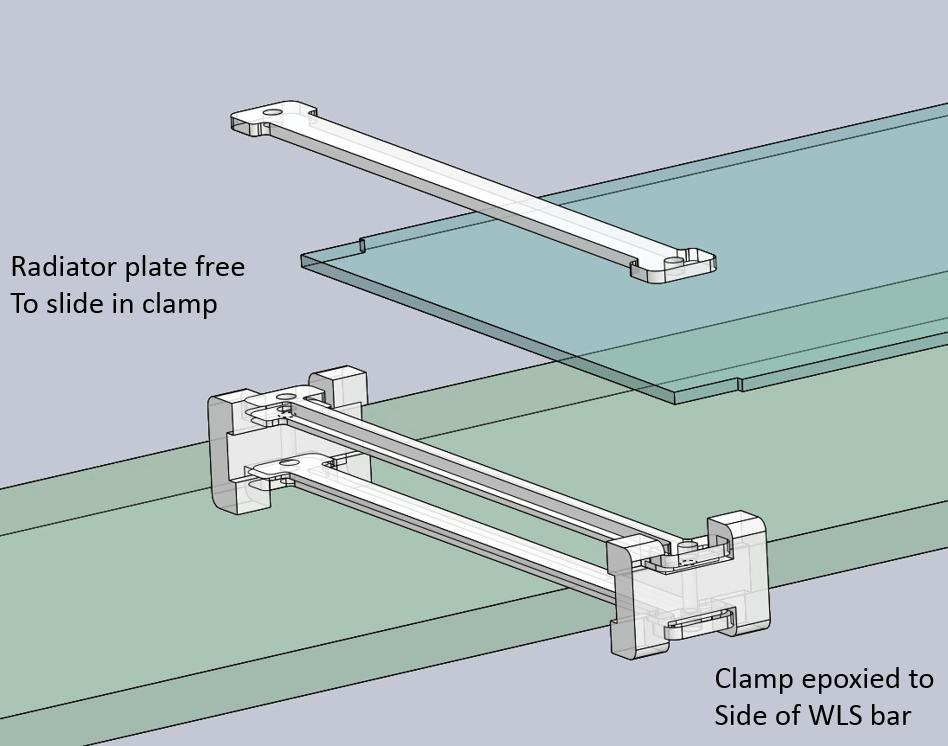
\includegraphics[width=0.5\columnwidth]{pds-DoubleShiftLG-PlateMounting.jpg}
\end{dunefigure}


\subsubsection{\color{red}\bf ARAPUCA}
\label{ssec:fdsp-pd-pc-prod-arapuca}
\metainfo{\color{red} Content needed: (2 pages) Machado}



%%%%%%%%%%%%%%%%%%%%%%%%%%%%%%%%%%
%\subsection{PD Mounting in APA Frames}
\subsection{APA Frame Mounting Structure and Module Fixing}	
\label{sec:fdsp-pd-assy-frames}
%\todo{\color{blue} Content:  Warner}

Photon detector (PD) modules are inserted into the APA frames through ten slots 
(five on each side of the APA frame) and are supported in place inside the frame in 
stainless steel guide channels.  The slot dimensions for the protoDUNE APA frames 
were 108.0~mm X 19.2~mm wide (see Figure~\ref{}).  The guide channels are pre-positioned into 
the APA frame prior to applying the wire shielding mesh to the APA frames, and are
not accessible following wire wrapping.

\fixme{Insert Dave's PD Mounting rails in APA frame mpicture}

Following insertion, the PD modules are fixed in place in the APA frame using
 two stainless steel captive screws, as shown in Figure~\ref{}).

\fixme{Insert Dave's PD Mounting screws mpicture}

\subsubsection{Cryogenic thermal contraction}

Bar-style PD modules are structurally composed of primarily polycarbonate and 
acrylic, which have significantly different shrinkage factors compared to the 
stainless steel APA and PD support frames (see Table 1).

\begin{dunetable}[Shrinkage of Photon Detector Materials.]
{|c|c|}
{tbl:fdsfpdshrink}
{Shrinkage of Photon Detector Materials}
Material Shrinkage Factor (m/m) & $206^{\circ}$C Drop\\ \toprowrule
Stainless Steel (304) & $2.7\times10^{-3}$\\ \colhline
FR-4 G-10 (In-plane) & $2.1\times10^{-3}$\\ \colhline
Polystyrene (Average) & $1.5\times10^{-2}$\\ \colhline
Acrylic and Polycarbonate (Average) & $1.4\times10^{-2}$\\ \colhline
\end{dunetable}

These differences in thermal expansion (or contraction in this case) were 
important to keep in mind during design of the PD module supports.  
Mitigation for these varying contractions are detailed in Table 2:

\begin{dunetable}[Relative Shrinkage of PD components and APA frame, and mitigations]
{|p{0.2\textwidth}|p{0.2\textwidth}|p{0.5\textwidth}l}
{tbl:fdsfpdshrinkeffects}
{Relative Shrinkage of PD components and APA frame, and mitigations}
\textbf{Interface} & \textbf{Relative shrinkage} & \textbf{Mitigation} \\ \toprowrule
PD Length to APA width & PD shrinks \SI{25.7}{mm} Relative to APA frame & PD affixed only at one end of APA frame, free to contract at other end \\ \colhline
Width of PD in APA Slot & PD shrinks \SI{1.2}{mm}  relative to slot width & Photon detector not constrained in C-channels. C channels and tolerances designed to contain module across thermal contraction range \\ \colhline
Width of SiPM mount board ({\it Hover board}) to stainless steel frame & Stainless frame shrinks \SI{0.06}{mm}  more than PCB & Diameter of shoulder screws and FR-4 board clearance holes selected to allow for motion \\ \colhline
Width of SiPM mount board relative to polycarbonate mount block & Polycarbonate block shrinks \SI{1}{mm} more than PCB & Allowed for in clearance holes in SiPM mount board \\ \colhline
\end{dunetable}

\subsubsection{PD Mount Frame Deformation under static PD load}

FEA modeling of the PD support structure was conducted to study static deflection 
prior to building prototypes.  Modeling was conducted in both the vertical
 orientation (APA upright, as installed in cryostat) and also flat.  
Basic assumptions used were fully-supported fixed end conditions for the rails, 
uniform loading of 3X PD mass (5 kg) along rails.  
Prototype testing confirmed these calculations.

\fixme{Insert Dave's 4 deflection pictures here}
%\fixme{Same for bars and ARAPUCAs}

%%%%%%%%%%%%%%%%%%%%%%%%%%%%%%%%%%
\subsection{Photosensor Modules}
\label{sec:fdsp-pd-assy-psm}
%\todo{\color{blue} Content: Zutshi}

The Silicon Photomultiplier analog signal will be ganged on the detector inside the
LAr volume. Passive and active ganging schemes are under consideration. Some passive
ganging (sensors put in parallel) schemes have been examined and are being installed inside
protoDUNE (see \fixme{Fig. yyy)}. The key point for parallel passive ganging in terms of 
maintaining signal-to-noise as devices are ganged together is the terminal capacitance of the 
sensors. This characteristics can therefore play an important in device selection or on
the flip side in determining the maximum ganging possible. In this scheme the 
ganged analog signals are then brought out via long cables (~25 m) for digitization outside
the cryostat. This is currently being done in protoDUNE using teflon ethernet CAT6 cables.

An interesting alternative option that may provide more flexibility in terms of the level of
photosensor ganging possible and also obviate the need for carrying analog signals of long cables
is the so-called active ganging option where the amplifiers and ADCs sit on the board carrying 
the photosensors inside the LAr volume. This option however brings, in all the reliability and long-term
stability issues related to cold electronics into play. While active ganging prototypes are under study 
the design cannot be considered to be at a mature stage at this point and schedule and technical
considerations may influence how far this promising option can be pursued.

In any case, the SiPMs will need to be surface-mounted on a PCB that can mate efficiently with the photon
collector options. protoDUNE will provide a wealth of operational experience and information on
such a design with at least a passive ganging board. It is already clear, however, that some R$\&$D is needed 
in optimizing the connectors to be used to couple the cable to the board and understanding the 
mechanical stresses involved in the SiPM-PCB-Connector system (with a varying CTEs) as it
is cooled (or cycled) to cryogenic temperatures.

\fixme{Just cold boards?}

%%%%%%%%%%%%%%%%%%%%%%%%%%%%%%%%%%
%\subsection{(Common Tooling} -- Probably not worth bothering about, except for QA/QC scanners, etc.
%\label{sec:fdsp-pd-assy-ct}
%\fixme{\color{blue} Content:  Warner}
%\fixme{Is there common tooling or is described separately in the PC section?}

%%%%%%%%%%%%%%%%%%%%%%%%%%%%%%%%%%
%\subsection{Assembly Procedures}
%\label{sec:fdsp-pd-assy-ap}
%\metainfo{\color{blue} Content: Cavanna/Whittington/Machado}

%PC assembly modules (ready for APA installation).

%\fixme{Can we have a single section that describes how the bars and/or ARAPUCA are assembled into PC modules or do we need a separate subsub(!)section for each?}

%\subsubsection{Dip-Coated Light Guide Modules (2 pages)}
%\label{ssec:fdsp-pd-pc-assy-bar1}

%\subsubsection{Double-Shift Light Guide Modules (2 pages)}
%\label{ssec:fdsp-pd-pc-assy-bar2}

%\subsubsection{ARAPUCA Modules (2 pages)}
%\label{ssec:fdsp-pd-pc-assy-arapuca}


%%%%%%%%%%%%%%%%%%%%%%%%%%%%%%%%%%
\subsection{Electronics}
\label{sec:fdsp-pd-assy-pde}
%\metainfo{\color{red}  Content: (2 pages) Moreno/Franchi/Djurcic}
%\todo{\color{blue}  Content: Moreno/Franchi/Djurcic}

The nature of research work and wide variety of developments necessitates a flexible manufacturing process, without compromising on the basic elements of workmanship. The circuit design is done in accordance with mutually agreed-upon specification documents. Printed circuit board (PCB) layout is performed in accordance with IPC specifications. Bare PCB manufacturing requirements are embedded within the Gerber file fabrication documents (e.g. layers, spacing, impedance, finish, testing, etc.). Components are assembled onto circuit using either trained Photon Detector Consortium  technical staff or by external assembly vendors, based upon volume, in accordance with per-design assembly specification documents. Testing occurs at labs and universities within Photon Detector Consortium in accordance with a per-design test procedure that typically includes a mix of manual, semi-automatic and automated testing in an engineering test bench followed by overall characterization in a system- or subsystem-test stand.

\begin{itemize}
\item Components: Schematic capture is done using appropriate tools (such as OrCAD 16.6. or similar toolset) available within design facility. Design is hierarchical with common front-end page referenced multiple times to ensure all input channels are identical. Schematic contains complete bill-of-materials (BOM) including all mechanical parts. Subversion repository is typically used for version control and backup. Multiple internal design reviews held before schematic is released to layout. The bill of materials is stored directly within schematic, extracted to Excel when ordering parts. Every part is specified by both manufacturer and distributor information. Distributor information may be overridden by technician at order time due to price and/or availability. Standard search engines such as Octopart, ECIA and PartMiner are used to check price/availability across all standard distributors. A parts availability check review is performed prior to handoff from schematic to layout; as required obsolete or long lead time parts were removed from design and replaced. BOM information will include dielectric, tolerance, temp. coefficient, voltage rating and size (footprint) to ensure all parts are fully described.
\item Boards: With respect to printed-circuit-board (PCB) there are standard tools (such as Allegro toolset) available for the layout job. Conventional PCBs are realized as multi-layer, controlled impedance board with many sets of delay-matched nets. In usual practice the complete impedance and delay characteristics calculated within layout tool and crosschecked by PCB vendor prior to manufacture. In usual procedure, a competitive bid between multiple previously qualified vendors is used, with a full electrical and impedance testing required. Multiple internal design reviews are held prior to release of design.
\item Cable plant: Cabling will be designed under considerations of the APA space and in close work with the TPC electronics to avoid cross-talk effects.  Manufacturing or purchase of cable will be evaluated based on cost and prospects of the Electronics Working Group.   
\item Manufacturer list: In addition to the general laboratory procedures for quality assurance, the Electronics Working Group will follow the general practice of using only those printed circuit board manufacturers and external assembly vendors whose workmanship and facilities have been personally inspected by members of the Electronics Working Group. All external assemblers are required to quote in accordance with an Assembly Specification document describing the IPC class and specific solder chemistry requirements of the design. The Bill of Materials document will need to show selected and alternate suppliers for every component of the front-end boards.
\end{itemize}

It is also mandatory to discuss the firmware specifications. Front-end electronics firmware will be specified iteratively with collaboration. The electronics working group within will be responsible to respond to requests for additional firmware development, including for example, modifications to timing interface, modifications to trigger interface, and implemented sensitivity to in-spill vs. not-in-spill conditions. Documents describing firmware architecture for each major change will be written and distributed to photon detector and DAQ working groups before implementation. Front-End electronics User's Manual containing all details of new firmware will be distributed with production units when manufactured.

With the mechanical assembly of electronics readout boards it is a custom to use  AutoCAD with Allegro (as PCB layout tool). All relevant dimensions of PC board including connector and indicator placement extracted from Allegro as base DXF file from which overall exploded mechanical diagram of chassis and other mechanical parts is made. Mechanical items such as shield plates will be provided as well. It is assumed that the front-end chassis will made by external vendors (one for chassis, one for front/back panels) from AutoCAD drawings provided by Electronics Working Group.

%%%%%%%%%%%%%%%%%%%%%%%%%%%%%%%%%%
% Combined into single QAQC section
%\subsection{QA}
%\label{sec:fdsp-pd-assy-qa}
%\metainfo{\color{blue} Content:  (2 pages) - Warner}

%\begin{itemize}
%\item Sub-assemblies- same for all modules.
%\item Completed modules- largely same for different option, at least for TP.
%\end{itemize}

